\section{The Lipkin-Meshkow-Glick model}

One of problem that many-body physics encounter in complex, real world, system is the fact that the many-body Schrödinger equation isn't exactly solvable. This may require either to approximate the Schrödinger equation or limit the number of particles in a system. Therefor it is more common to test many-body methods on simplified models where the exact solution is available without approximation. One of these models is the Lipkin-Meshkow-Glick model, abbreviated LMG or Lipkin in this thesis, first introduced in the 1960's \cite{LIPKIN1965188}.
\subsection{The model system}

The idea behind the LMG model is to have two energy levels separated by an energy-value $\varepsilon$, one just below the Fermi level and one just above. In our case we fill up the base energy level with any number of particles, which then can be excited up to the second energy level. \ref{fig:lipkinnumbered} shows a visualized example with two particles:

\begin{figure}[H]
    \centering
    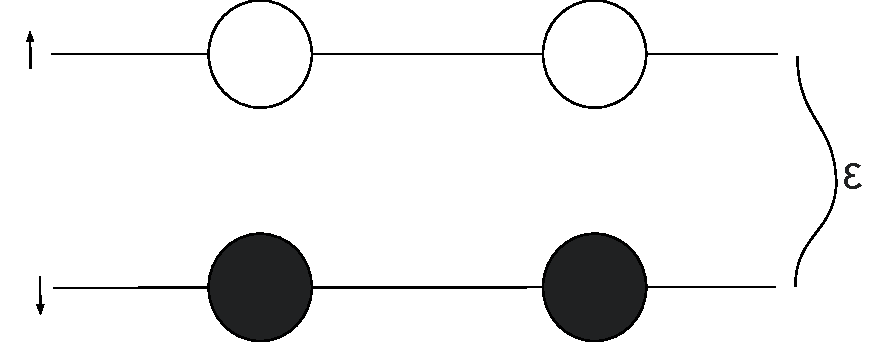
\includegraphics[width=0.7\textwidth]{Figures/Drawn/Lipkin/Lipkinstart22.pdf}
    \caption{The LMG model with two particles and two holes where the particles can move between the two layers. The two levels are separated by a constant $\varepsilon$. }
    \label{fig:lipkinnumbered}
\end{figure}

For a N-fermion system the levels are N-fold degenerate, represented by the different positions the particles can be in in \ref{fig:lipkinnumbered}, with two characteristic quantum numbers associated with each particle. The $\sigma$ quantum number is assumed to be $-1$ in the lower level and $+1$ in the higher level, which can be seen as particle spin. We will use $p$ to denote the degenerate state in which a particle resides in. So $\sigma$ denotes which level the particle is on and $p$ denotes where in that level it resides. The Hamiltonian proposed by Lipkin, Glick and Meshkow is as follows:

\begin{equation} \label{eq:creationanhilHamiltonian}
    H = \sum_{p\sigma} \left ( \frac{1}{2} \sigma \varepsilon \right ) \hc{a}{p\sigma}\op{a}{p\sigma} + \frac{V}{2}\sum_{pp'\sigma} \hc{a}{p\sigma} \hc{a}{p'\sigma} \op{a}{p'-\sigma}\op{a}{p-\sigma} + \frac{W}{2} \sum_{pp'\sigma} \hc{a}{p\sigma} \hc{a}{p'-\sigma} \op{a}{p'\sigma}\op{a}{p-\sigma} \; , 
\end{equation}

where the operators $\hc{a}{p\sigma}$ creates and $\op{a}{p\sigma}$ destroys a particle in the energy level associated with $\sigma$ and in the $p$ position within that level. As an example, if we start out with two particles in the lower level:

\begin{figure}[H]
    \centering
    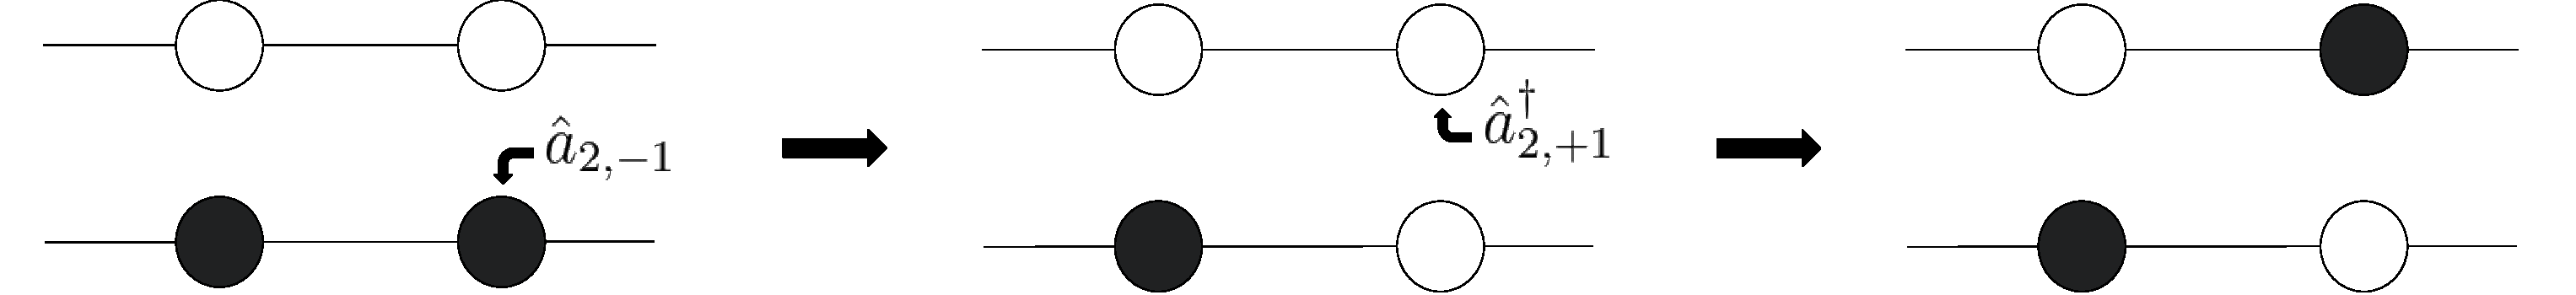
\includegraphics[width=\textwidth]{Figures/Drawn/Lipkin/lipkinexcited.pdf}
    \caption{Two particles in the $\sigma = -1$ level filling out the $p = 1$ and $p=2$ state of the LMG model. The particle at $p = 2$ and $\sigma = -1$ is destroyed and then a particle is created at $p=2 \; , \; \sigma = +1$.}
    \label{fig:lipkinbase}
\end{figure}

Here we excite one of the particles in the lower layer up to the $\sigma = +1$ layer by destroying and then creating a particle. The Hamiltonian has three parts. Firstly we have the single-particle energy of each particle in the system. Then there is a term that moves pairs of particle from one level to another, with an interaction strength proportional to $V$. Lastly we have a term that scatters a pair of particles, with an interaction strength proportional to $W$, exciting one up and de-exciting another.

\subsection{Rewriting the Hamiltonian}

An advantage of the LMG model is the fact that the two-body interaction does not change the value of $p$. Together with the two-valued $\sigma$, each particle can only exist in two possible states. This suggests to use the quasi-spin operators to rewrite the Hamiltonian. These quasi-spin operators are defined as follows:

\begin{equation}
J_{\pm} = \sum_p a_{p\pm}^\dagger a_{p\mp},
\label{eq:Jpm} \;, 
\end{equation}

\begin{equation} 
J_{z} = \frac{1}{2}\sum_{p,\sigma} \sigma a_{p\sigma}^\dagger a_{p\sigma},
\label{eq:Jz}\; , 
\end{equation}

\begin{equation} 
J^{2} = J_+ J_- + J_z^2 - J_z,
\label{eq:J2} \; ,
\end{equation}

where the $+, -$ indicates the quantum number $\sigma = \left \{ +1, -1\right \}$ as associated with spin up and spin down respectively. The $\op{J}{+}$ accounts for the energy of a particle being excited up a level, the $\op{J}{-}$ accounting for a particle falling down a level. While the $\op{J}{z}$ takes into account the difference in single-particle energy of the two energy levels. All for each degenerate states $p$. Following the calculations from the lecture notes by M.H Hjensen\cite{LipkinRewrite} we show that these obey the commutation relations for angular momentum. 

$$\begin{align*}
[J_z,J_\pm] &= J_z J_\pm - J_\pm J_z \\
%
&= \left( \frac{1}{2}\sum_{p,\sigma} \sigma a_{p\sigma}^\dagger a_{p\sigma} \right)
\left( \sum_{p'} a_{p'\pm}^\dagger a_{p'\mp} \right) -
\left( \sum_{p'} a_{p'\pm}^\dagger a_{p'\mp} \right)
\left( \frac{1}{2}\sum_{p,\sigma} \sigma a_{p\sigma}^\dagger a_{p\sigma} \right) \\
&= \frac{1}{2} \sum_{p,p',\sigma} \sigma \left( a_{p\sigma}^\dagger a_{p\sigma} a_{p'\pm}^\dagger a_{p'\mp} - a_{p'\pm}^\dagger a_{p'\mp} a_{p\sigma}^\dagger a_{p\sigma} \right).
\end{align*}$$

And with the relations

\begin{equation}
\{ a_l,a_k \} = 0, \label{eq:al,ak} \; ,
\end{equation}
\begin{equation} 
\{ a_l^\dagger , a_k^\dagger \} = 0, \label{eq:ald,akd}\;, 
\end{equation}

\begin{equation} 
\{ a_l^\dagger , a_k \} = \delta_{lk}, \label{eq:ald,ak} \;,
\end{equation}

we can move the operators to match in order of the products:

\begin{align*}
[J_z,J_\pm] &= \frac{1}{2} \sum_{p,p',\sigma} \sigma \left(
a_{p\sigma}^\dagger a_{p\sigma} a_{p'\pm}^\dagger a_{p'\mp} -
a_{p'\pm}^\dagger \left( \delta_{p' p} \delta_{\mp \sigma} - a_{p\sigma}^\dagger a_{p'\mp} \right) a_{p\sigma} \right) \\
&= \frac{1}{2} \sum_{p,p',\sigma} \sigma \left(
a_{p\sigma}^\dagger a_{p\sigma} a_{p'\pm}^\dagger a_{p'\mp} -
a_{p'\pm}^\dagger \delta_{p' p} \delta_{\mp \sigma} a_{p\sigma} +
a_{p'\pm}^\dagger a_{p\sigma}^\dagger a_{p'\mp} a_{p\sigma} \right), \\
\end{align*}

which gives us

\begin{align*}
[J_z,J_\pm]
&= \frac{1}{2} \sum_{p,p',\sigma} \sigma \left(
a_{p\sigma}^\dagger a_{p\sigma} a_{p'\pm}^\dagger a_{p'\mp} -
a_{p'\pm}^\dagger \delta_{pp'} \delta_{\mp \sigma} a_{p\sigma} +
a_{p\sigma}^\dagger a_{p'\pm}^\dagger a_{p\sigma} a_{p'\mp} \right) \\
&= \frac{1}{2} \sum_{p,p',\sigma} \sigma \left(
a_{p\sigma}^\dagger a_{p\sigma} a_{p'\pm}^\dagger a_{p'\mp} -
a_{p'\pm}^\dagger \delta_{pp'} \delta_{\mp \sigma} a_{p\sigma} +
a_{p\sigma}^\dagger \left( \delta_{pp'} \delta_{\pm \sigma} - a_{p\sigma} a_{p'\pm}^\dagger \right) a_{p'\mp} \right) \\
&= \frac{1}{2} \sum_{p,p',\sigma} \sigma \left(
a_{p\sigma}^\dagger \delta_{pp'} \delta_{\pm \sigma} a_{p'\mp} -
a_{p'\pm}^\dagger \delta_{pp'} \delta_{\mp \sigma} a_{p\sigma} \right). \\
\end{align*}

And we can shorten it further by comparing it to \ref{eq:Jpm}.

\begin{align*}
[J_z,J_\pm] &= \frac{1}{2} \sum_p \left(
(\pm 1) a_{p\pm}^\dagger a_{p\mp} - (\mp 1)
a_{p\pm}^\dagger a_{p\mp} \right) =
\pm \frac{1}{2} \sum_p \left(
a_{p\pm}^\dagger a_{p\mp} + (\pm 1)
a_{p\pm}^\dagger a_{p\mp} \right) \\
&= \pm \sum_p a_{p\pm}^\dagger a_{p\mp} = \pm J_\pm,
\end{align*}

Further we can use \ref{eq:Jpm} to compute the next relation

\begin{align*}
[J_+,J_-] &= J_+ J_- - J_- J_+ \\
&= \left( \sum_p a_{p'+}^\dagger a_{p-} \right)
\left( \sum_{p'} a_{p'-}^\dagger a_{p'+} \right) -
\left( \sum_{p'} a_{p'-}^\dagger a_{p'+} \right)
\left( \sum_p a_{p+}^\dagger a_{p-} \right) \\
&= \sum_{p,p'} \left(
a_{p'+}^\dagger a_{p-} a_{p'-}^\dagger a_{p'+} -
a_{p'-}^\dagger a_{p'+} a_{p+}^\dagger a_{p-} \right) \\
&= \sum_{p,p'} \left(
a_{p'+}^\dagger a_{p-} a_{p'-}^\dagger a_{p'+} -
a_{p'-}^\dagger \left( \delta_{++} \delta_{pp'} -
a_{p+}^\dagger a_{p'+} \right) a_{p-} \right) \\
&= \sum_{p,p'} \left(
a_{p'+}^\dagger a_{p-} a_{p'-}^\dagger a_{p'+} -
a_{p'-}^\dagger \delta_{pp'} a_{p-} +
a_{p'-}^\dagger a_{p+}^\dagger a_{p'+} a_{p-} \right) \\
&= \sum_{p,p'} \left(
a_{p'+}^\dagger a_{p-} a_{p'-}^\dagger a_{p'+} -
a_{p'-}^\dagger \delta_{pp'} a_{p-} +
a_{p+}^\dagger a_{p'-}^\dagger a_{p-} a_{p'+} \right) \\
&= \sum_{p,p'} \left(
a_{p'+}^\dagger a_{p-} a_{p'-}^\dagger a_{p'+} -
a_{p'-}^\dagger \delta_{pp'} a_{p-} +
a_{p+}^\dagger \left( \delta_{--} \delta_{pp'} -
a_{p-} a_{p'-}^\dagger \right) a_{p'+} \right) \\
&= \sum_{p,p'} \left(
a_{p+}^\dagger \delta_{pp'} a_{p'+} -
a_{p'-}^\dagger \delta_{pp'} a_{p-} \right), \\
\end{align*}

which gives us

$$[J_+,J_-] = \sum_p \left(
a_{p+}^\dagger a_{p+} -
a_{p-}^\dagger a_{p-} \right) = 2J_z,$$

and we have that

$$[J^2, J_\pm] = [J_+ J_- + J_z^2 - J_z, J_\pm] =
[J_+ J_-, J_\pm] + [J_z^2, J_\pm] - [J_z, J_\pm].$$

Together with the relations

\begin{equation}
[AB,C] = A[B,C] + [A,C]B, \label{eq:ab,c} \;\end{equation}

\begin{equation} 
[A,BC] = [A,B]C + B[A,C], \label{eq:a,bc} \; ,
\end{equation}

we get

$$[J^2, J_\pm] =
J_+ [J_-,J_\pm] + [J_+,J_\pm] J_- + J_z [J_z,J_\pm] + [J_z,J_\pm] J_z - [J_z,J_\pm].$$

This can further be used 

\begin{align*}
[J^2, J_+] &= -2J_+ J_z + J_z [J_z,J_+] + [J_z,J_+] J_z - [J_z,J_+] \\
&= -2J_+ J_z + J_z J_+ + J_+ J_z - J_+ \\
&= -2J_+ J_z + J_+ + J_+ J_z + J_+ J_z - J_+ = 0,
\end{align*}

and that

\begin{align*}
[J^2, J_-] &= 2J_z J_- + J_z [J_z,J_-] + [J_z,J_-] J_z - [J_z,J_-] \\
&= 2J_z J_- - J_z J_- - J_- J_z + J_- \\
&= J_z J_- - (J_z J_- + J_-) + J_- = 0.
\end{align*}

Lastly we have
\begin{align*}
[J^2,J_z] &= [J_+ J_- + J_z^2 - J_z, J_z] \\
&= [J_+ J_-, J_z] + [J_z^2, J_z] - [J_z, J_z] \\
&= J_+ [J_-, J_z] + [J_+,J_z] J_- \\
&= J_+ J_- - J_+ J_- = 0 \; ,
\end{align*}

which completes the set of relations:

\begin{equation}
[J_z, J_\pm] = \pm J_\pm, \label{eq:kJzJpm} \,
\end{equation}
\begin{equation} 
[J_+, J_-] = 2J_z, \label{eq:kJpJm} \,
\end{equation}
\begin{equation} 
[J^2, J_\pm] = 0, \label{eq:kJ2Jpm} \, 
\end{equation}
\begin{equation} 
[J^2,J_z] = 0, \label{eq:kJ2Jz} \; .
\end{equation}

Together with the number operator:

\begin{equation}
N = \sum_{p,\sigma} a_{p\sigma}^\dagger a_{p\sigma}.
\label{eq:N} \; ,
\end{equation}

we can go through each term of the Hamiltonian separately. The first part, $H_0$, is simple to see can be written as:

\begin{equation}
H_0 = \varepsilon J_z.
\label{eq:H0ny} \; .
\end{equation}

The $H_1$ part of the Hamiltonian can be rewritten using the relations \ref{eq:al,ak},\ref{eq:ald,akd} and \ref{eq:ald,ak}:

\begin{align*}
H_1 &= \frac{1}{2} V \sum_{p,p',\sigma}
a_{p\sigma}^\dagger a_{p'\sigma}^\dagger a_{p'-\sigma} a_{p-\sigma} \\
&= \frac{1}{2} V \sum_{p,p',\sigma}
-a_{p\sigma}^\dagger a_{p'\sigma}^\dagger a_{p-\sigma} a_{p'-\sigma} \\
&= \frac{1}{2} V \sum_{p,p',\sigma}
-a_{p\sigma}^\dagger \left( \delta_{pp'} \delta_{\sigma -\sigma} - a_{p-\sigma} a_{p'\sigma}^\dagger \right) a_{p'-\sigma} \\
&= \frac{1}{2} V \sum_{p,p',\sigma}
a_{p\sigma}^\dagger a_{p-\sigma} a_{p'\sigma}^\dagger a_{p'-\sigma} \\
\end{align*}

And we get

\begin{align*}
H_1 &= \frac{1}{2} V\sum_{p,p'}
a_{p+}^\dagger a_{p-} a_{p'+}^\dagger a_{p'-} +
a_{p-}^\dagger a_{p+} a_{p'-}^\dagger a_{p'+} \\
&= \frac{1}{2} V \left[ \sum_p \left( a_{p+}^\dagger a_{p-} \right)
\sum_{p'} \left( a_{p'+}^\dagger a_{p'-} \right) +
\sum_p \left( a_{p-}^\dagger a_{p+} \right)
\sum_{p'} \left( a_{p'-}^\dagger a_{p'+} \right) \right] \\
&= \frac{1}{2} V \left[ J_+ J_+ + J_- J_- \right] = \frac{1}{2} V \left[ J_+^2 + J_-^2 \right] ,
\end{align*}

For the final part, $H_2$, we have

\begin{align*}
H_2 &= \frac{1}{2} W \sum_{p,p',\sigma}
a_{p\sigma}^\dagger a_{p'-\sigma}^\dagger a_{p'\sigma} a_{p-\sigma} \\
&= \frac{1}{2} W \sum_{p,p',\sigma}
-a_{p\sigma}^\dagger a_{p'-\sigma}^\dagger a_{p-\sigma} a_{p'\sigma} \\
&= \frac{1}{2} W \sum_{p,p',\sigma}
-a_{p\sigma}^\dagger \left( \delta_{pp'} \delta_{-\sigma -\sigma} -
a_{p-\sigma} a_{p'-\sigma}^\dagger \right) a_{p'\sigma} \\
&= \frac{1}{2} W \sum_{p,p',\sigma}
-a_{p\sigma}^\dagger \delta_{pp'} a_{p'\sigma} +
a_{p\sigma}^\dagger a_{p-\sigma} a_{p'-\sigma}^\dagger a_{p'\sigma} \\
&= \frac{1}{2} W \left( -\sum_{p,\sigma}
a_{p\sigma}^\dagger a_{p\sigma} +
\sum_{p,p',\sigma} a_{p\sigma}^\dagger a_{p-\sigma} a_{p'-\sigma}^\dagger a_{p'\sigma} \right) \\
\end{align*}

and with the number operator it becomes

\begin{align*}
\sum_{p,p',\sigma} a_{p\sigma}^\dagger a_{p-\sigma} a_{p'-\sigma}^\dagger a_{p'\sigma}
&= \sum_{p,p'} a_{p+}^\dagger a_{p-} a_{p'-}^\dagger a_{p'+} +
a_{p-}^\dagger a_{p+} a_{p'+}^\dagger a_{p'-} \\
&= \sum_p \left( a_{p+}^\dagger a_{p-} \right)
\sum_{p'} \left( a_{p'-}^\dagger a_{p'+} \right) +
\sum_p \left( a_{p-}^\dagger a_{p+} \right)
\sum_{p'} \left( a_{p'+}^\dagger a_{p'-} \right) \\
&= J_+ J_- + J_- J_+,
\end{align*}

Summing the parts up we have that, using these quasi-spin operators, we can rewrite the Hamiltonian as:

\begin{equation}\label{eq:quasiHamilt}
    H = \varepsilon \op{J}{z} + \frac{V}{2} \left ( \op{J}{+}\op{J}{+}  + \op{J}{-}\op{J}{-} \right ) + \frac{W}{2} \left ( -N + \op{J}{+} \op{J}{-} + \op{J}{-}\op{J}{+} \right )
\end{equation}

\subsection{Analytical Solution}

For an exact solution of the LMG model one can use the full configuration interaction theory described in section \ref{sec:fci}. However, for a given total spin $J$ the spin of a state can overlap with systems with fewer particles. For example, a system with $J=2$ and another with $J = 1$ can both have the same spin projection $J_z=-1$ as seen below.

\begin{figure}[H]
\centering
\begin{subfigure}{.5\textwidth}
  \centering
  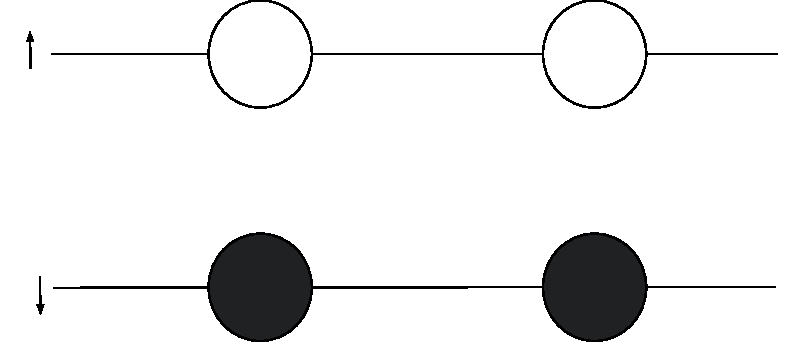
\includegraphics[width=.6\textwidth]{Figures/Drawn/Lipkin/j=1.pdf}
  \caption{$J=1$, $J_z = -1$}
  \label{fig:J=1}
\end{subfigure}%
\begin{subfigure}{.5\textwidth}
  \centering
  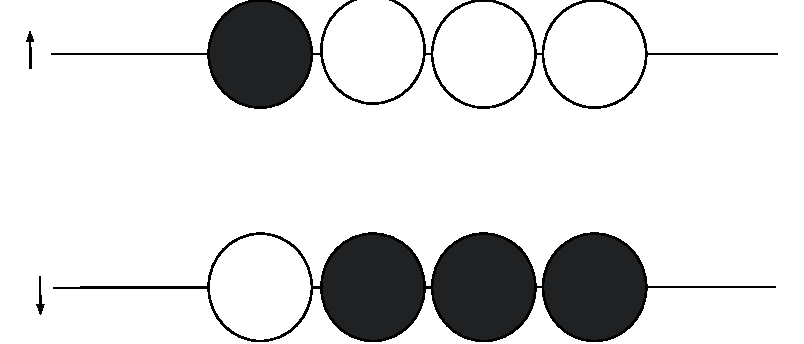
\includegraphics[width=.6\textwidth]{Figures/Drawn/Lipkin/j=2.pdf}
  \caption{$J=2$, $J_z=-1$}
  \label{fig:J=2}
\end{subfigure}
\caption{Two systems with different total spin but both are in a state where $J_z=-1$.}
\end{figure}

Therefor a more complete Hamiltonian would differentiate between these states. For a four-particle system we would then have 

\begin{equation}
    H_{4} = \begin{bmatrix}
        H_{J=2} &  & \text{\Large0}\\
         & H_{J=1} & \\
        \text{\Large0} & & H_{J=0}
    \end{bmatrix} \; . 
\end{equation}

Since the Hamiltonian commutes with $J^2$,

\begin{equation}
    \left [ H, J^2\right ] = 0 \;,
\end{equation}

$J$ is a good quantum number and all other elements in the $H_4$ Hamiltonian becomes zero. As a diagonal block matrix we can then instead diagonalize the $J$-specific Hamiltonians separately. For $J=2$ we construct the hamiltonian matrix with:

$$J_{2, z} = \begin{bmatrix} 
  2 & 0 & 0 & 0 & 0 \\
  0 & 1 & 0 & 0 & 0 \\
  0 & 0 & 0 & 0 & 0 \\
  0 & 0 & 0 & -1 & 0 \\
  0 & 0 & 0 & 0 & 1 \end{bmatrix}$$

$$J_{2, +} = \begin{bmatrix} 
  0 & 2 & 0 & 0 & 0 \\
  0 & 0 & \sqrt{6} & 0 & 0 \\
  0 & 0 & 0 & \sqrt{6} & 0 \\
  0 & 0 & 0 & 0 & 2 \\
  0 & 0 & 0 & 0 & 0 \end{bmatrix}$$

$$J_{2, -} = \begin{bmatrix} 
  0 & 0& 0 & 0 & 0 \\
  2  & 0 & 0 & 0 & 0 \\
  0 &\sqrt{6} & 0 & 0 & 0 \\
  0 & 0 & \sqrt{6}& 0 & 0\\
  0 & 0 & 0 & 2 & 0 \end{bmatrix} \; ,$$

and we get
\begin{equation}
H_{J = 2} =
\begin{bmatrix}
-2\varepsilon & 0 & \sqrt{6}V & 0 & 0 \\
0 & -\varepsilon + 3W & 0 & 3V & 0 \\
\sqrt{6}V & 0 & 4W & 0 & \sqrt{6}V \\
0 & 3V & 0 & \varepsilon + 3W & 0 \\
0 & 0 & \sqrt{6}V & 0 & 2\varepsilon
\end{bmatrix}
\label{eq:HJ=2} \; ,
\end{equation}

If we the diagonalize this matrix we get the following eigenvalues for $\varepsilon = 1$ and $W = 0$.

\begin{figure}[H]
    \centering
    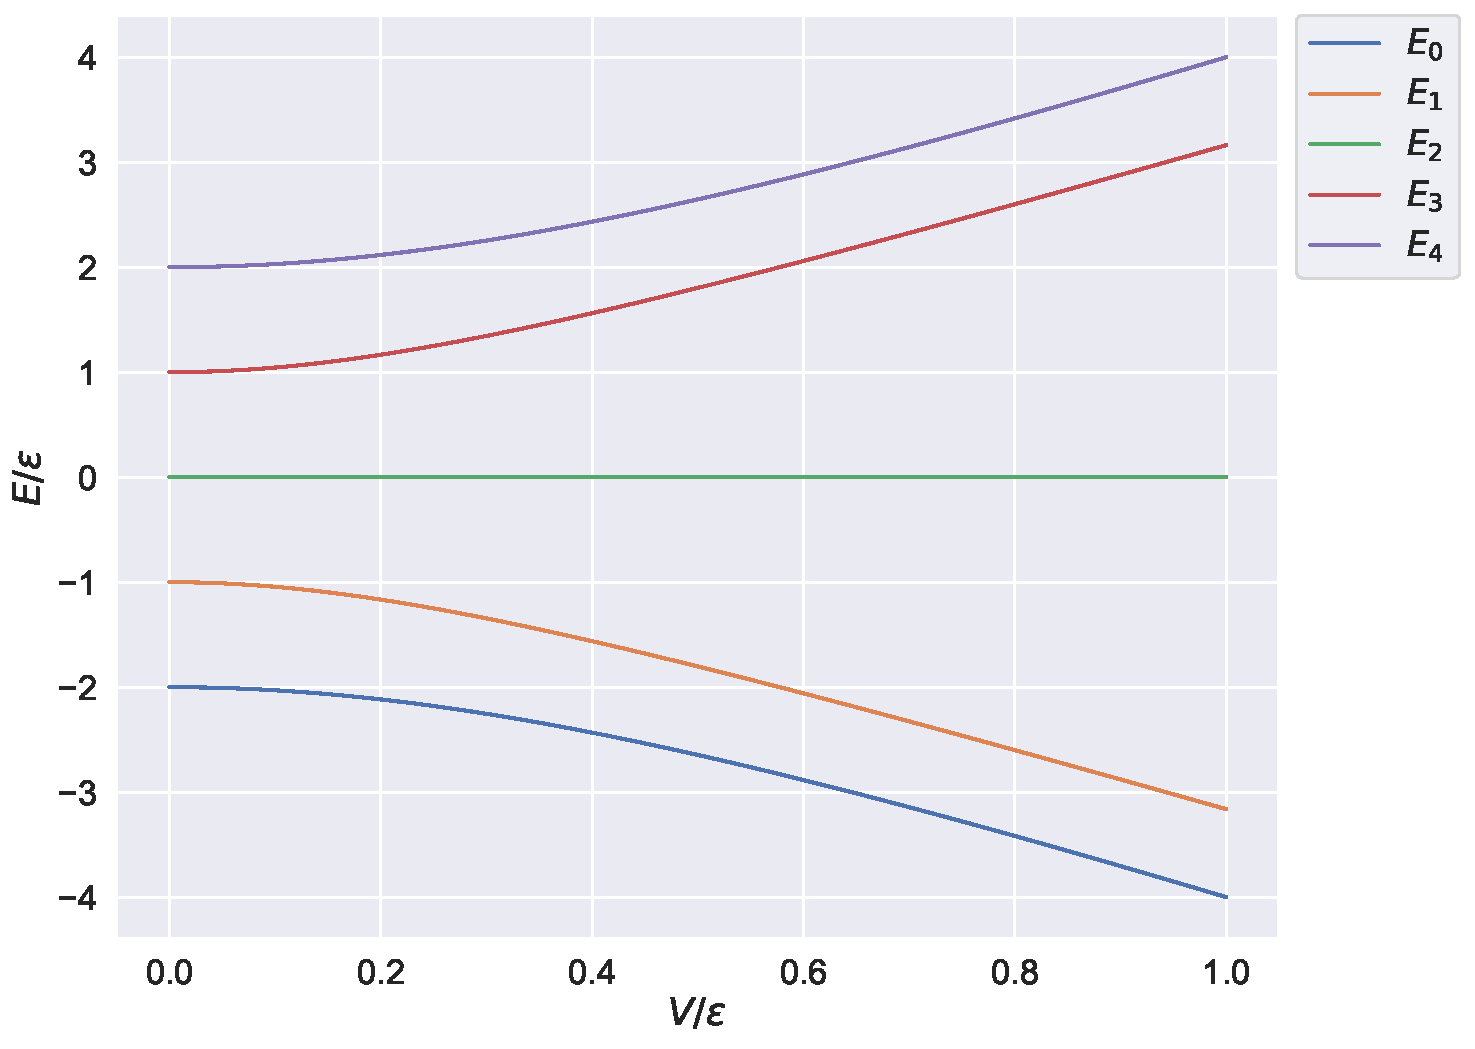
\includegraphics[width=\textwidth]{Figures/Plots/Lipkin/J2_true.pdf}
    \caption{The analytical solution for the LMG model with total spin $J=2$, $\varepsilon = 1$ and $W = 0$.}
    \label{fig:J2_true}
\end{figure}

And for $J=1$:

\begin{figure}[H]
    \centering
    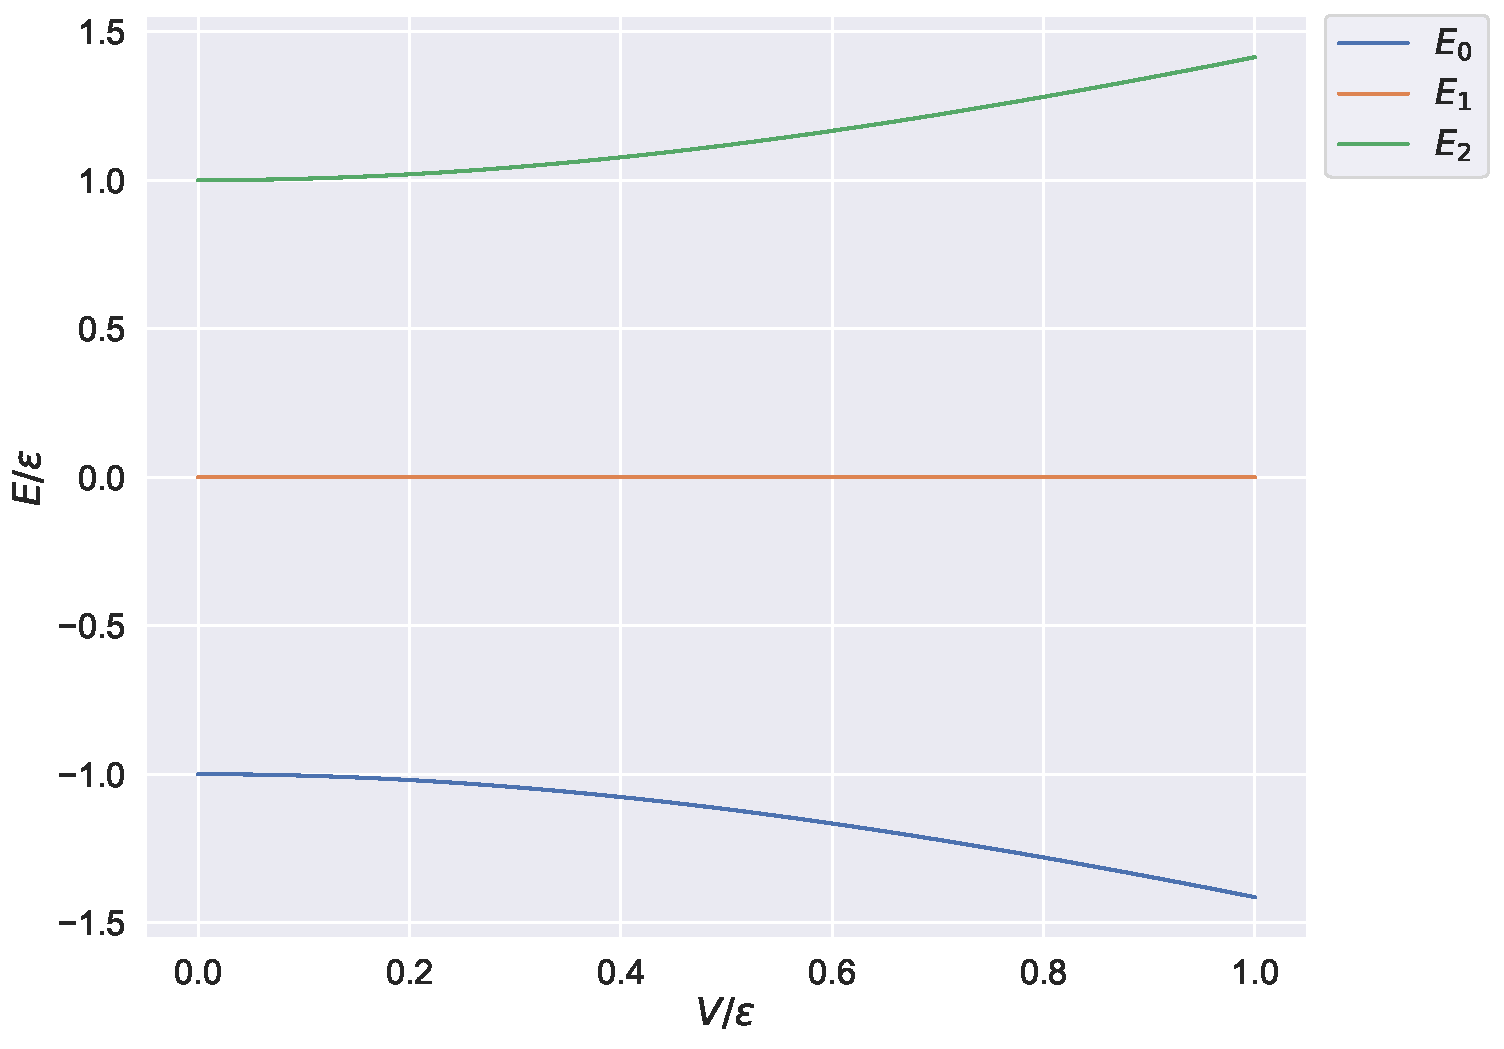
\includegraphics[width=\textwidth]{Figures/Plots/Lipkin/J1_true.pdf}
    \caption{The analytical solution for the LMG model with total spin $J=1$, $\varepsilon = 1$ and $W = 0$.}
    \label{fig:J1_true}
\end{figure}




